 
 The state diagram of the LoPy is shown in figure:
\begin{figure}[H]
\centering
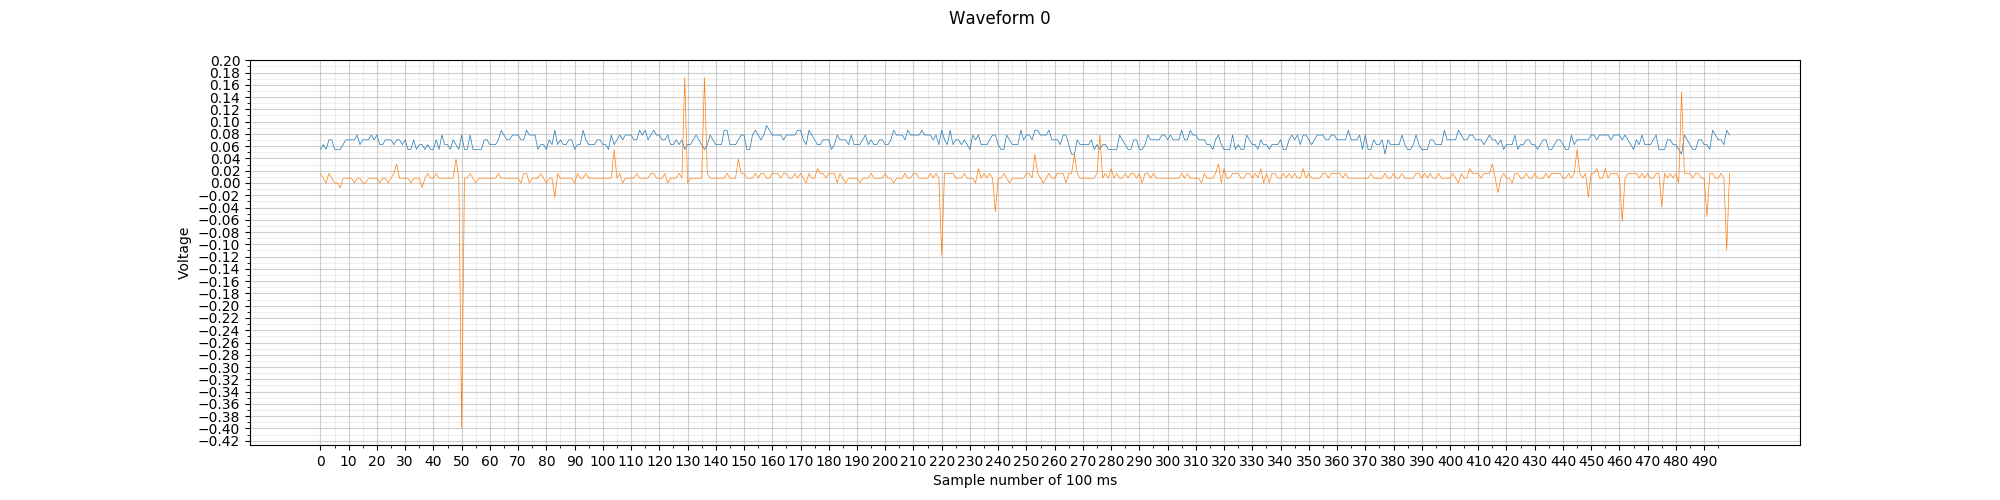
\includegraphics[height=4.5cm]{Project_Report/Images/pythonwaveform.png}
\caption{State diagram of the LoPy during a positional fix request}
\label{fig:LoPystate}
\end{figure}


 
 
 The average current consumption is then calculated for each waveform by using Ohm's law.The python script uses a simple energy model to calculate the energy consumption over a fix period. A fix period is defined as the duration the microcontroller use to acquire a fix:
\begin{equation}
E_{fixperiod} = P_{fixperiod}*T_{fixperiod}
\end{equation}
During a fix period, the microcontroller transitions between the states in \ref{fig:LoPystate}. The total energy consumption $E_{fixperiod}$ can then be written as the sum of the energy of each state:

\begin{equation}
E_{fixperiod} = P_{Idle}*T_{Idle} + P_{Acquisition}*T_{Acquisition} + P_{Tracking}*T_{Tracking} + P_{Deepsleep}*T_{Deepsleep}
\end{equation}

The total energy consumption over a duration t is given by the energy consumption of a fix period multiplied by the number of periods during the duration t.

\begin{equation}
 E_{total} = E_{fixperiod}* \frac{t}{fixperiod}
\end{equation}

The python scripts generates an Excel sheet with the data:

\begin{figure}[H]
\centering
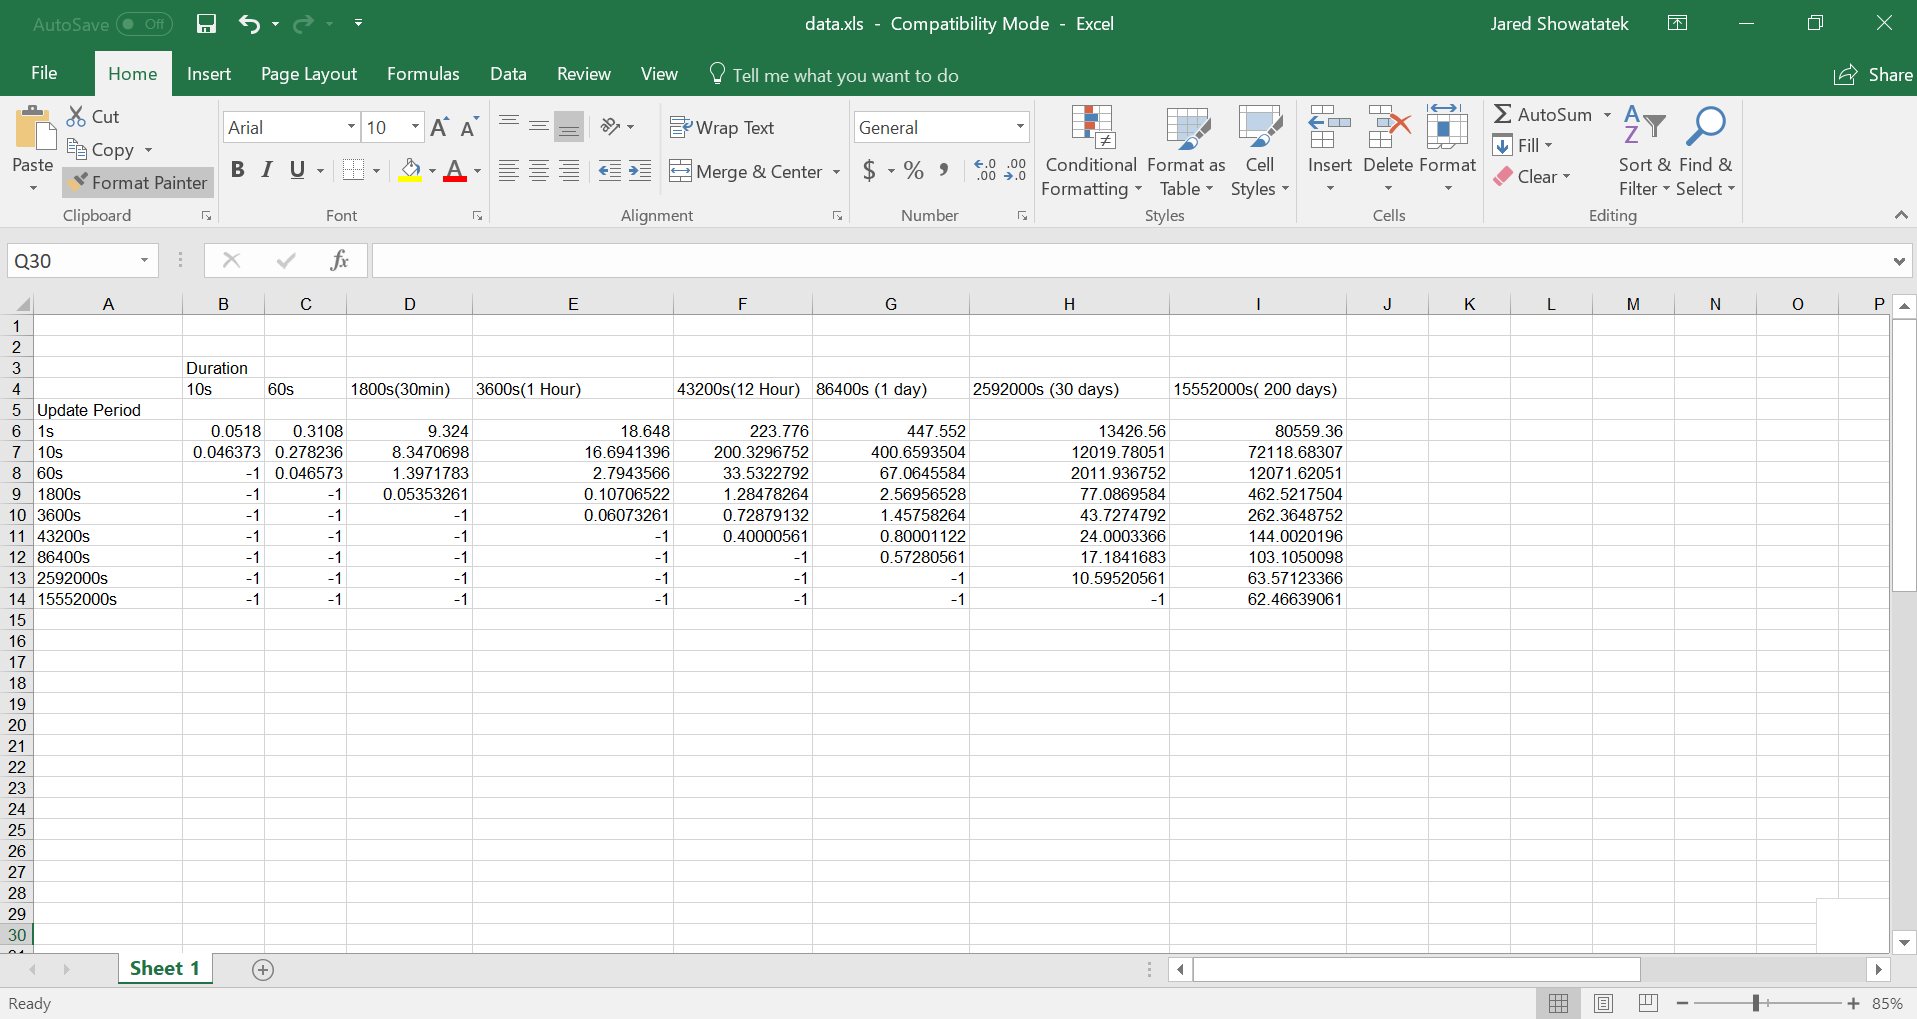
\includegraphics[height=4.5cm]{Project_Report/Images/Excel_sample.PNG}
\caption{Figure showing the generated Excel sheet}
\label{fig:Excelsample}
\end{figure}


